\newpage
\section{Funktionale Anforderungen}
Im folgenden Abschnitt betrachten wir die funktionalen Anforderungen an die Drunken-Jukebox. Dabei unterscheiden wir zwischen den Benutzerrollen Admin (dem Gastgeber) und Party-People (dem Gast).  

\subsection{Anwendungsfälle}
\subsubsection{Admin}
Für den Admin haben wir zwei Anwendungsfälle identifiziert. Als Gastgeber ist er für das Starten und Beenden einer Party verantwortlich. Darüber hinaus verwaltet er die Songsammlung, aus der Songs für die entsprechende Party ausgewählt und abgespielt werden können.

\begin{figure}[H]
\centering
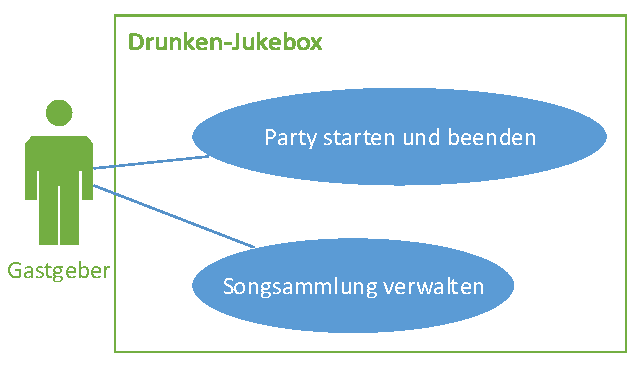
\includegraphics[width=0.75\linewidth]{Bilder/AdminUseCase}
\caption{Anwendungsfälle des Admins}
\label{fig:AdminUseCase}
\end{figure}

\newpage
\subsubsection{Party-People}
Die Anforderungen aus Sicht der Party-People sind etwas umfangreicher. Als Gast der Party möchte er die Playlist und den aktuellen gespielten Song abrufen können. Innerhalb der Playlist möchte er die Songs bewerten und darüber hinaus seine bisherigen Bewertungen einsehen. Des Weiteren möchte er seinen Betrunkenheitsgrad melden und einsehen können.

\begin{figure}[H]
\centering
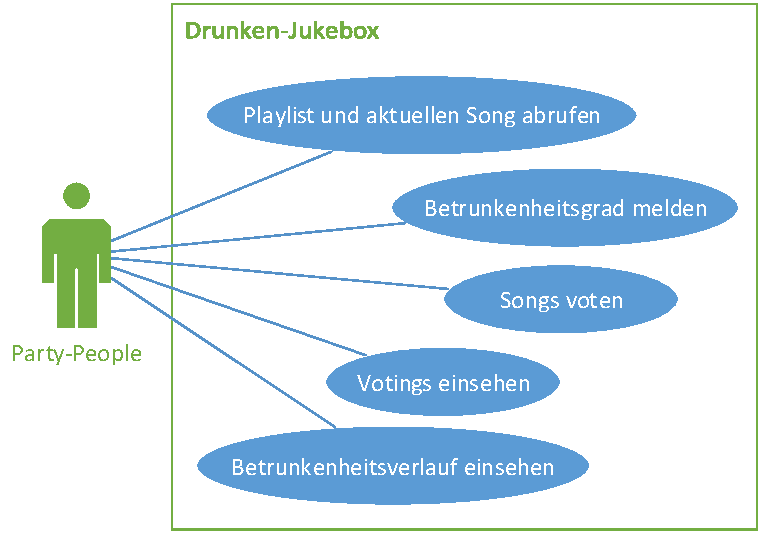
\includegraphics[width=0.95\linewidth]{Bilder/PartyPeopleUseCase}
\caption{Anwendungsfälle der Party-People}
\label{fig:PartyPeopleUseCase}
\end{figure}
